\documentclass[hidelinks]{ctexart}

\usepackage{van-de-la-illinoise}
\usepackage{cmbright}
\usepackage{nccmath}
\usepackage[paperheight=297mm,paperwidth=240mm,top=.2in,left=.1in,right=.1in,bottom=.2in, landscape]{geometry}
\usepackage{tensor}

\definecolor{graybg}{RGB}{228,235,243}
\definecolor{titlepurple}{RGB}{150,131,104}
\definecolor{shadegray}{RGB}{102,119,136}
\definecolor{itemgray}{RGB}{163,149,128}
\definecolor{mathnormalblack}{RGB}{0,0,0}
\pagecolor{graybg}

\setCJKmainfont{STHeitiSC-Light}
\setmainfont{Arial}

\usepackage{multicol}
\setlength{\columnsep}{.1in}

\newcommand{\raisedrule}[2][0em]{\qquad}
%\leaders\hbox{\rule[#1]{1pt}{#2}}\hfill}
\newcommand{\wdiv}{\,·\,}

\setlength{\parindent}{0pt}

\setCJKfamilyfont{pfsc}{STYuanti-SC-Regular}
\newcommand{\titlefont}{\CJKfamily{ttt}}
\setCJKfamilyfont{ttt}{STFangsong}
\newcommand{\mathtextfont}{\CJKfamily{ttt}}
\def\bili#1#2{#2}

\newdimen\indexlen
\def\newheader#1{%
\def\probindex{#1}
\setlength\indexlen{\widthof{\Large\color{titlepurple} #1\qquad}}
\vspace{1em}
{\Large\color{titlepurple} #1\qquad}
\raisebox{.5em}{\tikz \fill[titlepurple,opacity=.2,path fading=east] (0,0.05em) rectangle (\dimexpr\linewidth-\indexlen\relax,0em);}
}
\def\mathitem#1{\text{\color{itemgray}#1}}
\def\mathcomment#1{\text{\color{lightgray}\quad \texttt{\#}\kern-0pt#1}}
\def\mathheadcomment#1{\text{\color{lightgray}\texttt{\#}\kern-0pt#1}}
\def\midbreak{\smash{\raisebox{1.5em}{\smash{\tikz \path[opacity=.2,left color=white,right color=white,middle color=black] (0,0.05em) rectangle (\linewidth,0em);}}}
\vspace{-4em}}
\newtcolorbox{cheatresume}{enhanced, arc=.5pt, left=.5em, frame hidden, boxrule=0pt, colback=white, fuzzy halo=.05pt with lightgray, shadow={.4pt}{-.4pt}{0pt}{fill=shadegray,opacity=0.3}}

\usepackage{van-le-trompe-loeil}
\usetikzlibrary{matrix,positioning,fit}

\def\econfig#1{\immediate\write18{echo "#1" | python /Users/zechen/Documents/PhantasiaAcademia/electronconfig.py > electronsconfigtmp.tex}$\mathrm{3s^{1}\ 3p^{1}}$%
}

\usetikzlibrary{decorations.pathmorphing}

\tikzset{wavy/.style={decorate, decoration=snake}}

\begin{document}

\begin{multicols*}{3}[\centerline{\titlefont 量子論の基礎及び雑務}]
\raggedcolumns%
\newheader{\bili{}{言葉}}
\begin{cheatresume}
    \begin{flalign*}
        & \mathitem{Lyman} && n = 1 && \mathitem{s} && l= 0 && \mathitem{S\scriptsize(Sub II)} && n\mathrm{s}\mapsto 3\mathrm{p} \\
        & \mathitem{Balmer} && n = 2 && \mathitem{p} && l = 1 && \mathitem{P} && n\mathrm{p}\mapsto 3\mathrm{s} && \\
        & \+:c3l{$\mathitem{$H_\alpha$}\quad n:3\mapsto 2$} && \mathitem{d} && l = 2 && \mathitem{D\scriptsize(Sub I)} && n\mathrm{s}\mapsto 3\mathrm{p} \\
        & \mathitem{Paschen} && n = 3 && \mathitem{f} && l = 3 && \mathitem{F\scriptsize(Bergmann)} && n\mathrm{f}\mapsto 3\mathrm{d} \\
        & \+:c3l{$\mathitem{D線}\quad 3p \mapsto 3s$} && \+:c7l{\mathitem{Parahelium}\ ${^1S_0}$ \quad \mathitem{Orthohelium}\ ${^3S_1}$} && \\
        & \+:c7l{\mathitem{Gerade} \ $\Lambda\+_g_$ \ \mathitem{Ungerade}\ $\Lambda\+_u_$} && \+:c5l{\mathitem{s,S,$\sigma$,$\Sigma$}\ $\rightarrow $$l$,$L$,$\lambda$,$\Lambda$} \\
        & \+:c7l{\mathitem{OPQRS}\ ${J\downarrow_{-2,-1}}\uparrow^{0,+1,+2}$} && \+:c5l{\mathitem{KLM} \ $n=1,2,3$}
    \end{flalign*}
\end{cheatresume}
\newheader{Rutherford\bili{}{散乱}}
\begin{cheatresume}
    \begin{flalign*}
        & \mathheadcomment{以下に} && D = \rec{4\pi\epsilon_0}\frac{Z'Ze^2}{E} && \\
        & \mathitem{散乱角} && \cot \frac{\theta}{2} = \frac{2b}{D} \quad %{\color{lightgray}\bigg|}
         \mathitem{断面積} \quad \+d\Omega d\sigma = \frac{D^2}{16}\rec{\sin^4 \pare{\theta/2}} && \\
        & \mathitem{比率} && \frac{\rd{n}}{n\,\rd{\Omega}} = \frac{NtD^2}{16}\rec{\sin^4\pare{\theta/2}} && \\
        & && n\pare{\theta_1\sim\theta_2} = Nnt\pi \frac{D^2}{4}\pare{\cot^2 \frac{\theta_2}{2} - \cot^2 \frac{\theta_1}{2}} &&
    \end{flalign*}
\end{cheatresume}
\newheader{\bili{}{量子力学}}
\begin{cheatresume}
    \begin{flalign*}
        & \+:c5l{\mathitem{Schr\"odinger}\ $\displaystyle \brac{-\frac{\hbar^2}{2m}\laplacian + V}u = Eu$ \ \mathitem{確率流}\ $\displaystyle j = \frac{\hbar k}{m}\abs{A}^2$} \\
        & \+:c3{l}{$\mathitem{井戸型}\quad\displaystyle  T \approx 16\frac{E}{V_0}\pare{1-\frac{E}{V_0}}\exp\pare{-\frac{2a}{\hbar}\sqrt{2m\pare{V_0 - E}}}$} && \\
        & \mathitem{期待値} && \expc{Q} = \int \psi^*\cdot \hat Q \cdot \psi \,\rd{\tau} &&
    \end{flalign*}
    \midbreak
    \begin{flalign*}
        & \mathitem{角運動量} && \hat L^2 Y_{ml} = l\pare{l+1}\hbar^2 Y_{ml}\ {\color{lightgray}\vert}\ \hat L_z Y_{ml} = m\hbar Y_{ml} && \\
        & \mathitem{結合} && \+vJ = \+vL + \+vS && \\
        & && \quad J = \abs{L-S},\cdots,L+S,\quad M = -J,\cdots, J && \\
        & \mathitem{内積} && \+vS\cdot \+vL = \frac{\hbar^2}{2}\brac{j\pare{j+1} - s\pare{s+1} - l\pare{l+1}} &&
    \end{flalign*}
    \midbreak
    \begin{flalign*}
        & \mathitem{不確定性原理} && \Delta p_x \Delta x \ge \frac{\hbar}{2},\quad \Delta E \Delta t \ge \frac{\hbar}{2} &&
    \end{flalign*}
\end{cheatresume}
\columnbreak
\newheader{Bohr\bili{}{原子模型}}
\begin{cheatresume}
    \begin{flalign*}
        & \mathitem{軌道半径}\ r_n = \frac{4\pi\epsilon_0 \hbar^2}{Ze^2 m_\mu}n^2 \ \mathitem{エネルギー}\ E_n = -\half m_\mu c^2 \alpha^2 \frac{Z^2}{n^2} && \\
        & \mathitem{周回速度}\enspace v = \sqrt{\frac{Ze^2}{4\pi\epsilon_0 m_\mu r}} \enspace \mathitem{波数}\enspace \tilde{\nu} = Z^2R\pare{\rec{n^2} - \rec{m^2}} && 
    \end{flalign*}
\end{cheatresume}
\newheader{\bili{}{様々な基礎}}
\begin{cheatresume}
    \begin{flalign*}
        & \mathitem{Millikan油滴実験} && && \\
        & \mathitem{油滴半径}\ r = \sqrt{\frac{9\eta v_g}{2\pare{\rho - \rho_0 g}}} \ \mathitem{電荷量} \ e_k = \frac{4\pi \eta rl}{V}\pare{v_e + v_g} &&
    \end{flalign*}
    \midbreak
    \begin{flalign*}
        & \mathitem{光学} && && \\
        & \+:c5l{\smash{\raisebox{1.5em}{\rotatebox[origin=tl]{-90}{\mathitem{de Broglie}}}}\ $\displaystyle \begin{array}{@{}l}
            \lambda = \\
            \displaystyle =\frac{h}{p}
        \end{array}\begin{cases}
            \displaystyle \frac{h}{\sqrt{2mT}},\ \beta \ll 1\ \mathitem{$\gamma$}\ \displaystyle E = h\nu = \frac{hc}{\lambda}\quad p = \frac{E}{c} = \frac{h}{\lambda} \\
            \displaystyle \frac{hc}{E},\ \beta \sim 1,\ \mathitem{Compton}\ \displaystyle \Delta \lambda = \frac{h}{m_e c}\pare{1 - \cos\varphi}
        \end{cases}$} && \\
        & \mathitem{表面回折} \quad d \sin\theta = n\lambda\quad \mathitem{Bragg} \quad 2d\sin\theta = n\lambda &&
    \end{flalign*}
    \midbreak
    \begin{flalign*}
        & \mathitem{常用定数} && \frac{e^2}{4\pi\epsilon_0} = \SI{1.44}{\eV\cdot\nano\meter} && hc = \SI[inter-unit-product = \ensuremath{{}\cdot{}}]{1.24}{\nano\meter\kilo\eV} && \\
        & && m_e c^2 = \SI{0.511}{\mega\eV} && \hbar c = \SI[inter-unit-product = \ensuremath{{}\cdot{}}]{197}{\eV}{\nano\meter} &&
    \end{flalign*}
    \midbreak
    \begin{flalign*}
        & \mathitem{黒体放射} && && \\
        & \mathitem{Stefan} && R = \sigma T^4,\quad \sigma = \SI[inter-unit-product = \ensuremath{{}\cdot{}}]{5.6703e-8}{\watt\per\square\meter\per\kelvin\tothe{4}} && \\
        & \+:c5l{\mathitem{Wien}\ $\displaystyle \lambda\+_m_T = \SI[inter-unit-product = \ensuremath{{}\cdot{}}]{2.898}{\milli\meter\kelvin}$\ \mathitem{Planck} $\displaystyle u\pare{\lambda} = \frac{8\pi hc}{\lambda^5}\rec{e^{\beta h\nu} - 1}$ }
    \end{flalign*}
\end{cheatresume}
\newheader{\bili{}{選択律}}
\begin{cheatresume}
\begin{flalign*}
    & \mathitem{共用} && \sum \Delta l = \pm 1 && \\
    & && \Delta J = 0,\pm 1,\quad J=0\not\leftrightarrow 0 && \\
    & && \Delta M_J = 0,\pm 1 \mathcomment{$\Delta J=0$と\ } M_J=0\not\leftrightarrow 0  && \\
    & \mathitem{$LS$結合} && \Delta S = 0,\quad \Delta L = 0, \pm 1 && \\
    & \mathitem{$jj$結合} && \Delta j = 0,\pm 1 \mathcomment{遷移する電子} &&
\end{flalign*}
\end{cheatresume}
\columnbreak
\newheader{\bili{}{多電子原子}}
\begin{cheatresume}
    \begin{tabular}{@{}p{3cm}p{7cm}}
        \mathitem{電子配置} & \mathitem{Hund規則}\quad $\textcircled{\small{1}}\max S \Rightarrow \textcircled{\small{2}}\max L $ \\
        \+:r3{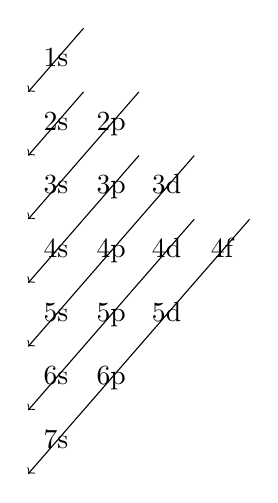
\begin{tikzpicture}[baseline={([yshift={-\ht\strutbox}]current bounding box.north)},outer sep=0pt,inner sep=0pt]
            \draw
            (0,0) node[minimum height=2.3em,minimum width=2em,anchor=north west] (1s) {1\strut s}
            (0,-2.3em) node[minimum height=2.3em,minimum width=2em,anchor=north west] (2s) {2\strut s}
            (2em,-2.3em) node[minimum height=2.3em,minimum width=2em,anchor=north west] (2p) {2\strut p}
            (0,-4.6em) node[minimum height=2.3em,minimum width=2em,anchor=north west] (3s) {3\strut s}
            (2em,-4.6em) node[minimum height=2.3em,minimum width=2em,anchor=north west] (3p) {3\strut p}
            (4em,-4.6em) node[minimum height=2.3em,minimum width=2em,anchor=north west] (3d) {3\strut d}
            (0,-6.9em) node[minimum height=2.3em,minimum width=2em,anchor=north west] (4s) {4\strut s}
            (2em,-6.9em) node[minimum height=2.3em,minimum width=2em,anchor=north west] (4p) {4\strut p}
            (4em,-6.9em) node[minimum height=2.3em,minimum width=2em,anchor=north west] (4d) {4\strut d}
            (6em,-6.9em) node[minimum height=2.3em,minimum width=2em,anchor=north west] (4f) {4\strut f}
            (0,-9.2em) node[minimum height=2.3em,minimum width=2em,anchor=north west] (5s) {5\strut s}
            (2em,-9.2em) node[minimum height=2.3em,minimum width=2em,anchor=north west] (5p) {5\strut p}
            (4em,-9.2em) node[minimum height=2.3em,minimum width=2em,anchor=north west] (5d) {5\strut d}
            (0,-11.5em) node[minimum height=2.3em,minimum width=2em,anchor=north west] (6s) {6\strut s}
            (2em,-11.5em) node[minimum height=2.3em,minimum width=2em,anchor=north west] (6p) {6\strut p}
            (0,-13.8em) node[minimum height=2.3em,minimum width=2em,anchor=north west] (7s) {7\strut s}
            ;
            \draw[->] (1s.north east) -- (1s.south west);
            \draw[->] (2s.north east) -- (2s.south west);
            \draw[->] (2p.north east) -- (3s.south west);
            \draw[->] (3p.north east) -- (4s.south west);
            \draw[->] (3d.north east) -- (5s.south west);
            \draw[->] (4d.north east) -- (6s.south west);
            \draw[->] (4f.north east) -- (7s.south west);
        \end{tikzpicture}}
     & $\begin{array}[t]{@{}l}
        \Rightarrow\textcircled{\small{3}} \begin{cases}
            \min J & \text{\color{lightgray}半数以下} \\
            \max J & \text{\color{lightgray}半数より多く} \\
        \end{cases}
    \end{array}$ \\
    & \raisebox{-.5em}{\mathitem{$LS$結合\hspace{1.8cm}$jj$結合}} \\
    & 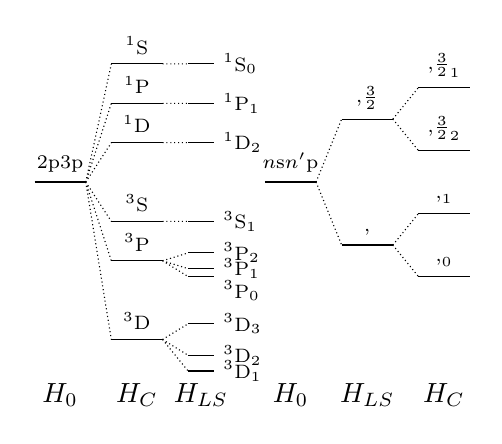
\begin{tikzpicture}[xscale=.65]
        \draw (0,0) -- (1,0)  node (2p3pr) {}  node[midway,above] {$\scriptstyle 2\mathrm{p} 3\mathrm{p}$}
        (1.5,0.5) node (1d){} -- (2.5,0.5) node (1dr) {} node[midway,above] {$\scriptstyle ^1\mathrm D$}
        (1.5,1) node (1p){} -- (2.5,1) node (1pr) {}  node[midway,above] {$\scriptstyle ^1\mathrm P$}
        (1.5,1.5) node (1s){} -- (2.5,1.5) node (1sr) {}  node[midway,above] {$\scriptstyle ^1\mathrm S$}
        (1.5,-0.5) node (3s){}  -- (2.5,-0.5)  node (3sr){}  node[midway,above] {$\scriptstyle ^3\mathrm S$}
        (1.5,-1) node (3p){}  -- (2.5,-1)  node (3pr){}  node[midway,above] {$\scriptstyle ^3\mathrm P$}
        (1.5,-2) node (3d){}  -- (2.5,-2)  node (3dr){}  node[midway,above] {$\scriptstyle ^3\mathrm D$}
        (3,0.5) node (1d2){}  -- (3.5,0.5) node[right] {$\scriptstyle ^1\mathrm D_2$}
        (3,1) node (1p1){} -- (3.5,1) node[right] {$\scriptstyle ^1\mathrm P_1$}
        (3,1.5) node (1s0){} -- (3.5,1.5) node[right] {$\scriptstyle ^1\mathrm S_0$}
        (3,-0.5) node (3s1){} -- (3.5,-0.5) node[right] {$\scriptstyle ^3\mathrm S_1$}
        (3,-0.9) node (3p2){} -- (3.5,-0.9) node[right] {$\scriptstyle ^3\mathrm P_2$}
        (3,-1.1) node (3p1){} -- (3.5,-1.1) node[right] {$\scriptstyle ^3\mathrm P_1$}
        (3,-1.2) node (3p0){} -- (3.5,-1.2) node[below right=-.2em and 0em] {$\scriptstyle ^3\mathrm P_0$}
        (3,-1.8) node (3d3){} -- (3.5,-1.8) node[right] {$\scriptstyle ^3\mathrm D_3$}
        (3,-2.2) node (3d2){} -- (3.5,-2.2) node[right] {$\scriptstyle ^3\mathrm D_2$}
        (3,-2.4) node (3d1){} -- (3.5,-2.4) node[right] {$\scriptstyle ^3\mathrm D_1$}
        ;
        \draw[densely dotted] (2p3pr.center) -- (1s.center)
        (2p3pr.center) -- (1p.center)
        (2p3pr.center) -- (1d.center)
        (2p3pr.center) -- (3s.center)
        (2p3pr.center) -- (3p.center)
        (2p3pr.center) -- (3d.center)
        (1sr.center) -- (1s0.center)
        (1pr.center) -- (1p1.center)
        (1dr.center) -- (1d2.center)
        (3sr.center) -- (3s1.center)
        (3pr.center) -- (3p2.center)
        (3pr.center) -- (3p1.center)
        (3pr.center) -- (3p0.center)
        (3dr.center) -- (3d3.center)
        (3dr.center) -- (3d2.center)
        (3dr.center) -- (3d1.center)
        ;
        %
        \draw (4.5,0) -- (5.5,0)  node (nsnpr) {}  node[midway,above] {$\scriptstyle n\mathrm{s} n'\mathrm{p}$}
        (6,0.8) node (halftrif){} -- (7,0.8) node (halftrifr) {}  node[midway,above] {$\scriptstyle \pare{\half,\frac{3}{2}}$}
        (6,-0.8) node (halfhalf){} -- (7,-0.8) node (halfhalfr) {}  node[midway,above] {$\pare{\scriptstyle \half,\half}$}
        (7.5,1.2) node (halftrif1){} -- (8.5,1.2) node[midway,above] {$\scriptstyle \pare{\half,\frac{3}{2}}_1$}
        (7.5,0.4) node (halftrif2){} -- (8.5,0.4) node[midway,above] {$\scriptstyle \pare{\half,\frac{3}{2}}_2$}
        (7.5,-1.2) node (halfhalf0){} -- (8.5,-1.2) node[midway,above] {$\scriptstyle \pare{\half,\half}_0$}
        (7.5,-0.4) node (halfhalf1){} -- (8.5,-0.4) node[midway,above] {$\scriptstyle \pare{\half,\half}_1$}
        ;
        \draw[densely dotted] (nsnpr.center) -- (halftrif.center)
        (nsnpr.center) -- (halfhalf.center)
        (halftrifr.center) -- (halftrif1.center)
        (halftrifr.center) -- (halftrif2.center)
        (halfhalfr.center) -- (halfhalf0.center)
        (halfhalfr.center) -- (halfhalf1.center)
        ;
        \draw (0.5,-2.7) node {$H_0$}
        (2,-2.7) node {$H_C$}
        (3.25,-2.7) node {$H_{LS}$}
        (5,-2.7) node {$H_0$}
        (8,-2.7) node {$H_C$}
        (6.5,-2.7) node {$H_{LS}$}
        ;
    \end{tikzpicture}
    \end{tabular}
    \begin{tabular}{@{}l}
        \mathitem{$LS$結合\wdiv Land\'e間隔則}\quad $\Delta E_J - \Delta E_{J-1} = \xi_{LS}\hbar^2 J$ \\
        \mathitem{$LS$結合\wdiv Slaterダイアグラム} \\
        \resizebox{\hsize}{!}{$\underbrace{\begin{array}{c|ccc}
    &   & M_S & \\
    \hline
    &   & 1   & \\
    & 1 & 2   & 1\\
M_L & 1 & 3   & 1\\
    & 1 & 2   & 1\\
    &   & 1   &
\end{array}}_{\displaystyle \text{\econfig{2p2}}} = \underbrace{\begin{array}{c|ccc}
    &   & M_S & \\
    \hline
    &   & 1   & \\
    &   & 1   & \\
M_L &   & 1   & \\
    &   & 1   & \\
    &   & 1   &
\end{array}}_{\displaystyle \ce{^1D}} + \underbrace{\begin{array}{c|ccc}
    &   & M_S & \\
    \hline
    &   &     & \\
    & 1 & 1   & 1 \\
M_L & 1 & 1   & 1 \\
    & 1 & 1   & 1 \\
    &   &     &
\end{array}}_{\displaystyle \ce{^3P}} + \underbrace{\begin{array}{c|ccc}
    &   & M_S & \\
    \hline
    &   &     & \\
    &   &     &   \\
M_L &   & 1   &   \\
    &   &     &   \\
    &   &     &
\end{array}}_{\displaystyle \ce{^1S}}$} \\
        \mathitem{$LS$結合\wdiv 2つの電子の場合}\quad $2\divs \pare{L+S}$ \\
        $\displaystyle n\mathrm{d}^2 \Rightarrow \begin{cases}
            S=0 \Rightarrow L=0,2,4:& ^1\mathrm G_4, ^1\mathrm D_2, ^1\mathrm S_0 \\
            S=1 \Rightarrow L=1,3:& ^3P_{2,1,0}, ^3F_{4,3,2}
        \end{cases}$ \\
        \mathitem{$LS$結合\wdiv 電子ー正孔対称性} \quad $\pare{nl}^{\nu} \cong \pare{nl}^{Y-\nu}$
    \end{tabular}
\begin{tabular}{@{}ll}
    \mathitem{Moseley法則} & {$\displaystyle {\tilde{\nu}\+_{K_{\mathnormal{\alpha}}}_}{} = R\pare{Z-1}^2\pare{\rec{1^2} - \rec{2^2}}$} \\
    & {$\displaystyle {\tilde{\nu}\+_{L_{\mathnormal{\alpha}}}_}{} = R\pare{Z-7.4}^2\pare{\rec{2^2} - \rec{3^2}}$}
\end{tabular}
\begin{tabular}{cc}
    \mathitem{特性X線} & \mathitem{Auger電子} \\
    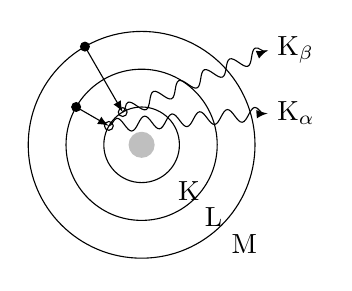
\begin{tikzpicture}[scale=0.8]
    \draw (0,0) circle (1.8);
    \draw (-45:1.8) node[below right] {M};
    \draw (0,0) circle (1.2);
    \draw (-45:1.2) node[below right] {L};
    \draw (0,0) circle (0.6);
    \draw (-45:0.6) node[below right] {K};
    \draw (0,0) node[circle,fill=lightgray] {};
    \draw[fill=black] (120:1.8) circle (0.07);
    \draw[fill=black] (150:1.2) circle (0.07);
    \draw (120:0.6) circle (0.07);
    \draw (150:0.6) circle (0.07);
    \draw[-latex] (120:1.8) -- (120:0.6);
    \draw[-latex] (150:1.2) -- (150:0.6);
    \draw[wavy, -latex] (120:0.6) -- (2,1.5) node[right] {$\mathrm{K}_\beta$};
    \draw[wavy, -latex] (150:0.6) -- (2,0.5) node[right] {$\mathrm{K}_\alpha$};
\end{tikzpicture} &
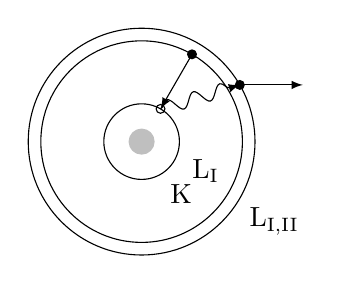
\begin{tikzpicture}[scale=0.8]
    \draw (0,0) circle (1.6);
    \draw (-30:1.6) node[above left] {L\textsubscript I};
    \draw (0,0) circle (1.8);
    \draw (-30:1.8) node[below right] {L\textsubscript {I,II}};
    \draw (0,0) circle (0.6);
    \draw (-60:0.6) node[below right] {K};
    \draw (0,0) node[circle,fill=lightgray] {};
    \draw[fill=black] (60:1.6) circle (0.07);
    \draw[fill=black] (30:1.8) circle (0.07);
    \draw (60:0.6) circle (0.07);
    \draw[-latex] (60:1.6) -- (60:0.6);
    \draw[wavy, -latex] (60:0.6) -- (30:1.8);
    \draw[-latex] (30:1.8) --++ (1,0);
\end{tikzpicture}
\end{tabular}


\end{cheatresume}

\end{multicols*}

\end{document}
